\documentclass[hyperref={xetex}]{beamer}
\title{Einführung in Matlab und Python - Einheit 4}
\subtitle{Polynome u. Interpolation, In- Output, Debugging}
\mode<article>
{
  \usepackage{fullpage}
  \usepackage{pgf}
  \usepackage{hyperref}
  \setjobnamebeamerversion{beamer}
}

\mode<presentation>
{
  %\usetheme{Frankfurt}
 %\usetheme{My}
  \usetheme{Madrid}
  % or ...
%\usecolortheme{seagull}
  %\setbeamercovered{transparent}
  %\setbeamercovered{dynamic}
  % or whatever (possibly just delete it)
}
\usenavigationsymbolstemplate{}
\usefonttheme{structurebold}
\usepackage{multimedia}
\usepackage{tikz}
\usepackage{fontspec,xunicode,xltxtra}
%\usepackage[scaled=.90]{helvet}
% Or whatever. Note that the encoding and the font should match. If T1
% does not look nice, try deleting the line with the fontenc.

\setbeamertemplate{footline}
{
\leavevmode
%\hbox{\begin{beamercolorbox}[wd=.5\paperwidth,ht=2.5ex,dp=1.125ex,
%leftskip=.3cm plus1fill,rightskip=.3cm]{author in head/foot}%
%    \usebeamerfont{author in head/foot}\insertshortauthor
%  \end{beamercolorbox}%
%  \begin{beamercolorbox}[wd=.5\paperwidth,ht=2.5ex,dp=1.125ex,leftskip=.3cm,
%rightskip=.3cm plus1fil]{title in head/foot}%
%    \usebeamerfont{title in head/foot}\insertshorttitle\hfill

\hfill\insertframenumber  \hspace{3pt}

%\inserttotalframenumber
%\hspace*{2ex}
%  \end{beamercolorbox}}%
  \vskip3pt%
}

%\usepackage[english]{babel}
\usepackage[ngerman]{babel}
\selectlanguage{ngerman}

%
% math/symbols
%
\usepackage{amssymb}
\usepackage{amsthm}
% \usepackage{latexsym}
\usepackage{amsmath}
%\usepackage{listings}
\usepackage[framed]{mcode}
%\usepackage{mcode}

\usepackage{mydef}
\usepackage{cmap} % you can search in the pdf for umlauts and ligatures
%\usepackage{colonequals} %corrects the definition-symbols \colonequals (besides others)
\title{Einführung in Matlab}
%
%\subtitle{Disputation} % (optional)

\author{Jochen Schulz}
% - Use the \inst{?} command only if the authors have different
%   affiliation.

\institute{Georg-August Universit\"at G\"ottingen \pgfimage[height=0.5cm]{../figures/unilogo3}}
% - Use the \inst command only if there are several affiliations.
% - Keep it simple, no one is interested in your street address.

\date{\today}

\subject{Einführung in Matlab}
% This is only inserted into the PDF information catalog. Can be left
% out. 



% If you have a file called "university-logo-filename.xxx", where xxx
% is a graphic format that can be processed by latex or pdflatex,
% resp., then you can add a logo as follows:

%\logo{\pgfimage[height=0.5cm]{figures/unilogo3}}


% Delete this, if you do not want the table of contents to pop up at
% the beginning of each subsection:
% \AtBeginSubsection[]
% {
%   \begin{frame}<beamer>
%     \frametitle{Aufbau}
%     \tableofcontents[currentsection,currentsubsection]
%   \end{frame}
% }

\AtBeginSection[]
{
  \begin{frame}<beamer>
    \frametitle{Aufbau}
    \tableofcontents[currentsection,currentsubsection]
  \end{frame}
}


\begin{document}



\begin{document}
\titlepage

\section{Polynome und Interpolation}

\subsection{Polynomiale Interpolation selbstgemacht}
% 
% Slide
% 
\begin{frame}[fragile]\frametitle{Polynomiale Interpolation}
\begin{columns}[b]
 \column{0.6\textwidth}
Suche ein Polynom vom Grad 3
\[ p(x)= p_0 +p_1 x +p_2 x^2 +p_3 x^3,  \]
 dass durch die vier Punkte
$(0,1)$, $(1,1)$, $(2,4)$, $(5,3)$
verläuft.
\column{0.4\textwidth}
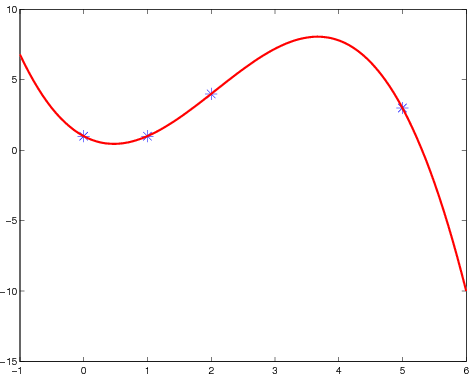
\includegraphics[width=\textwidth]{figures/grafik_6}
\end{columns}
$\Rightarrow  \alert{ p(0)=1, \ p(1)=1, \ p(2)=4, \ p(5)=3}$

$\Rightarrow \quad$ Lineares GLS \alert{ $Ap=b$} mit
{\scriptsize \[ A= \left( \begin{array}{cccc}
1 & 0 & 0 & 0\\
1 & 1 & 1 & 1\\
1 & 2 & 2^2 & 2^3 \\
1 & 5 & 5^2 & 5^3 \\
\end{array} \right), \
p=\left( \begin{array}{c} 
p_0 \\ p_1 \\ p_2 \\p_3\\
\end{array} \right),
\
b=\left( \begin{array}{c} 
1 \\ 1 \\ 4 \\ 3\\
\end{array} \right),
\]}  
\end{frame}
% 
% Slide
% 
\begin{frame}[fragile]\frametitle{Polynomiale Interpolation II}
Suche ein Polynom vom Grad n
\[ p(x)= p_0 +p_1 x +p_2 x^2 +p_3 x^3+ \dots +p_n x^n,  \]
 dass durch die  $n+1$ Punkte $(x_i,y_i)_{i=0}^n$
verläuft.\\[1cm]

\textbf{Beispiel}: Interpolation von
\[ (x_i,y_i)_{i=0}^{12} \]
mit \mcode{x=linspace(-5,5,13)} und $y_i=\frac{1}{1+x_i^2}$. 
\end{frame}
% 
% Slide
% 
\begin{frame}[fragile]\frametitle{Polynomiale Interpolation: Beispiel}
\begin{center}
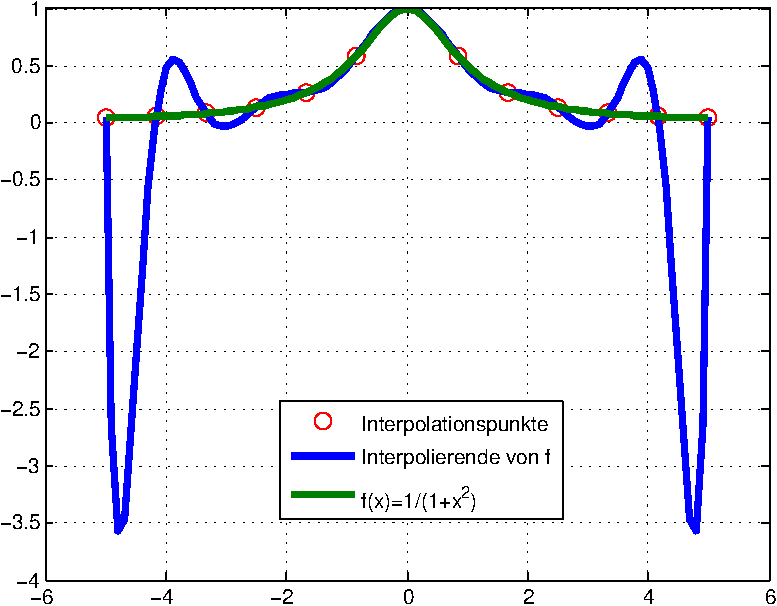
\includegraphics[width=0.8\textwidth]{figures/grafik_7}
\end{center}
\end{frame}
% 
% Slide
% 
\begin{frame}[fragile]\frametitle{Matlab: eigene Interpolation I}
\matinput{interpol2.m}
\end{frame}

% 
% Slide
% 
\begin{frame}[fragile]\frametitle{Matlab: eigene Interpolation II}
\matinput{interpol3.m}
\end{frame}
\begin{frame}[fragile]{Python: eigene Interpolation}
\begin{pyin}
def interpol2(x,y):
    A=vander(x)
    p=solve(A,y)
    return p  
x = linspace(-5,5,13)
y = 1/(1+x*x)
plot(x,y,'or',markersize=8)
p = interpol2(x,y)
x1 = linspace(-5,5,100)
y1 = ausw_poly2(p[::-1],x1)
y2 = 1/(1+x1*x1)
plot(x1,y1,x1,y2,linewidth=3)
xlim([-6,6])
grid('on'),box('on')
legend(('Interpolationspunkte','Interpolierende von f','$f(x)=1/(1+x^2)$'),loc='best')  
\end{pyin}
  
\end{frame}

\subsection{Polynome - built-in}
%
% Slide
%
\begin{frame}[fragile]\frametitle{Polynome}
Polynome 
\[ p(x)=p_1 x^n+ p_2 x^{n-1}+ \cdots + p_{n+1} \]
werden  durch einen Zeilenvektor $p=[p(1) \ p(2) \ \dots
\   p(n+1)]$ repr\"asentiert. \vspace*{0.5cm}\\

\alert{ Vorsicht:} Normalerweise werden Polynome in der Form
$\sum_{i=0}^n p_ix^i$ dargestellt. Dies ist hier invers!
\end{frame}
%
% Slide
%
\begin{frame}[fragile]\frametitle{Problemstellungen}
\begin{itemize}
\item [1.] \alert{ Auswerten:} Bei gegebenen Koeffizienten, das
  zugeh\"orige Polynom an bestimmten Stellen auswerten.
\item [2.] \alert{ Nullstellenbestimmung:} Bestimme zu gegebenen
  Koeffizienten die Nullstellen des zugeh\"origen Polynoms.
\item [3.]  \alert{ Interpolation}: Bestimme zu einer gegebenen Menge von
  Punkten $(x_i,y_i)_{i=0}^n$ ein Polynom $n$.-ten Grades, das durch
  diese Punkte verl\"auft.
\end{itemize}
\end{frame}
%
% Slide
%
\begin{frame}[fragile]\frametitle{Auswerten}
\begin{matlabin}
y = polyval(<p>,<x>)
\end{matlabin}
mit Koeffizientenvektor $p$ und Ort $x$ berechnet die Funktionswerte $y$.
($x$ kann eine Matrix sein)

\medskip
\alert{Beispiel:} $p(x):= x^3 - x^2 +1$\\
\begin{columns}[c]
\column{0.55\textwidth}
\begin{matlabin}
x = -2:0.1:2; 
y = polyval([1 -1 0 1],x); 
plot(x,y,'r--','Linewidth',3);
\end{matlabin}
\column{0.45\textwidth}
%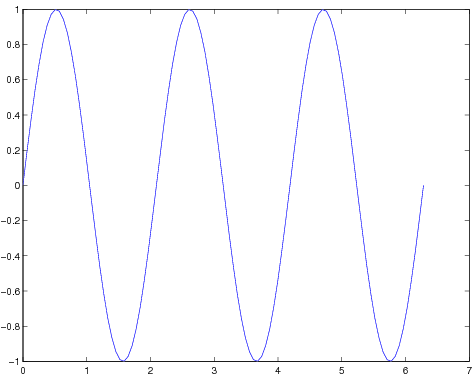
\includegraphics[width=5cm, height=3cm]{grafik_1}
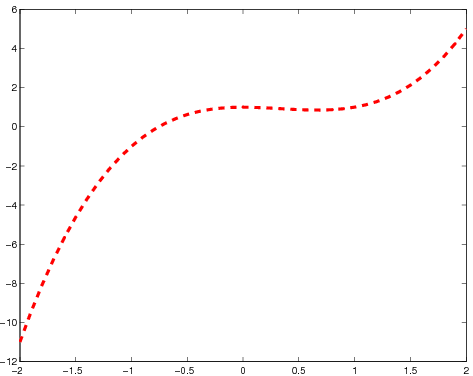
\includegraphics[width=\textwidth]{figures/polynom1}
\end{columns}
\end{frame}
%
% Slide
%
\begin{frame}[fragile]\frametitle{Bestimmung von Nullstellen}
\begin{matlabin}
z = roots(<p>)
\end{matlabin}
Nullstellen $z$ mit Koeffizientenvektor $p$.

\textbf{Beispiel:} \\
$p(x):= x^3 - x^2 +1$\\
\begin{columns}[c]
\column{0.58\textwidth}
\begin{matlabin}
roots([1 -1 0 1])
\end{matlabin}
\begin{matlab}
ans =
   0.8774 + 0.7449i
   0.8774 - 0.7449i
  -0.7549  
\end{matlab}
\begin{matlabin}
x = -1:0.1:1;
[X,Y] = meshgrid(x,x);
Z=abs(polyval([1 -1 0 1],X+i*Y)); 
surf(X,Y,Z)
\end{matlabin}
\column{0.43\textwidth}
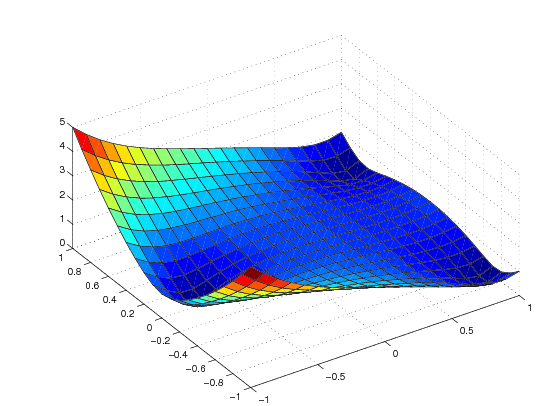
\includegraphics[width=\textwidth]{figures/polynom2}
\end{columns}
\end{frame}


\subsection{Interpolation}
% 
% Slide
%
\begin{frame}[fragile]\frametitle{Interpolation}
Suche zu  ein Polynom $p$ gegebenen Punkten $(x_i,y_i)_{i=0}^n$
$m$.-ten Grades
\begin{matlabin}
p = polyfit(x,y,m)
\end{matlabin}
\begin{itemize}
 \item $m=n$:\\ 
$p(x_i)=y_i$ f\"ur $i=0, \dots ,n$.
\item  $m<n$:\\ 
Least Square L\"osung, d.h. das Polynom $p$ der Ordnung $m$,
welches 
\[ 
\sum_{i=0}^n (p(x_i)-y_i)^2
\]
minimiert. 
\end{itemize}

\end{frame}

%
% Slide
%
\begin{frame}[fragile]\frametitle{Data Fitting}
\begin{matlabin}
yi = interp1(x,y,xi,<method>)
\end{matlabin}
\begin{pyin}
f = sp.interpolate.interp1d(x,y,kind=<method>)
yi = f(xi)
\end{pyin}
Dabei sind $(x,y)$ die gegebenen Punkte, $xi$ sind die Stellen, an die
die Interpolante berechnet wird und $yi$ sind die entsprechenden
Funktionswerte. 

\mcode{<method>}:
%{\scriptsize
\begin{tabular}{ll}
\mcode{'nearest'} &  stückweise konstante Approximation \\
\mcode{'linear'}  & Lineare Interpolation \\ 
\mcode{'spline'} & stückweise kubischer Spline (Matlab)\\
\mcode{'cubic'} & kubische Hermite Interpolation\\ 
\end{tabular}
%}
\end{frame}
%
% Slide
%
\begin{frame}[fragile]\frametitle{Beispiel}
\hfil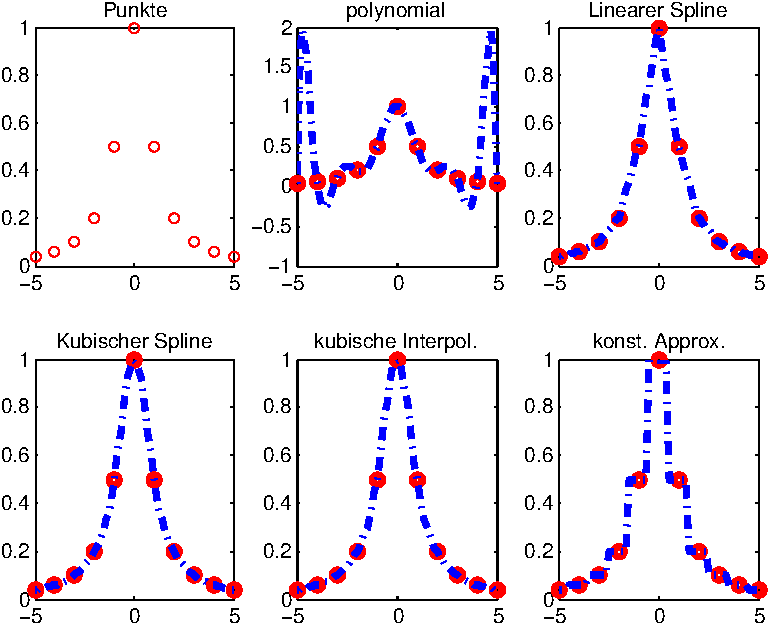
\includegraphics[width=0.8\textwidth]{figures/data_fitting}\hfil
\end{frame}
%
% Slide
%
\begin{frame}[fragile]\frametitle{Bemerkungen}
\begin{itemize}
\item Spline-interpolation: $u$ ($u \in C^2$,$u|_{[x_i,x_{i+1}]} \in \mathbb{P}_3$) \\
(Python) Splines durch spezialisierte Funktionen z.B. \isage{UnivariateSpline}) 
\item  (Matlab) Nur für die Spline-Methoden können   bei \mcode{interp1}  auch
  Stellen außerhalb des
  Interpolationsintervalls berechnet werden.
\item (Matlab) Data Fitting kann auch über die Oberfläche durchgeführt werden.
 Plotten Sie die Daten und wählen Sie \mcode{Basic Fitting} im Men\"u
 \mcode{Tools}. 

\end{itemize}
\end{frame}
%
% Slide
% 
% \begin{frame}[fragile]\frametitle{Lineare Regression}
% \begin{matlabin}
% % Example for Linear Regression 
% x = (1:0.5:4)';
% y = exp(x);
% plot(x,y,'o');
% hold on;
% pause;
% %--- Determine least square fit for
% 
% %    f(t)=a(1) + a(2) t + a(3) t^2
% 
% n=length(x);
% A = [ ones(n,1), x, x.^2 ];
% a = A \ y;
% %--- Plot new curve
% x1 = 1:0.1:4;
% y1 = a(1) + a(2)*x1 + a(3)*x1.^2;
% plot(x1,y1,'LineWidth',2)
% \end{matlabin}
% \end{frame}

\subsection{Interpolieren von 3D-Daten}

%
% Slide
% 
\begin{frame}[fragile]\frametitle{Nicht-reguläre Daten}
\begin{itemize}
\item Daten liegen h\"aufig in Form von Vektoren $(x,y,z)$ vor. Man m\"ochte
  eine Funktion $F$ mit $z(i) = F(x(i),y(i))$ plotten.
\item Befehle \mcode{surf} und \mcode{mesh} funktionieren nur wenn  die
  Einträge in $x$ und $y$ monoton sind und die Daten auf einem kartesischen
  Gitter vorliegen.
\item Ausweg: Interpolieren der Daten auf ein entsprechendes Gitter. 
\end{itemize}
\end{frame}
%
% Slide
% 
\begin{frame}[fragile]\frametitle{Beispiel}
\begin{matlabin}
load seamount
plot(x,y,'.','markersize',10)
\end{matlabin}
\begin{pyin}
x,y,z=loadtxt('seamount.csv',delimiter=',',unpack=True)  
\end{pyin}
\begin{center}
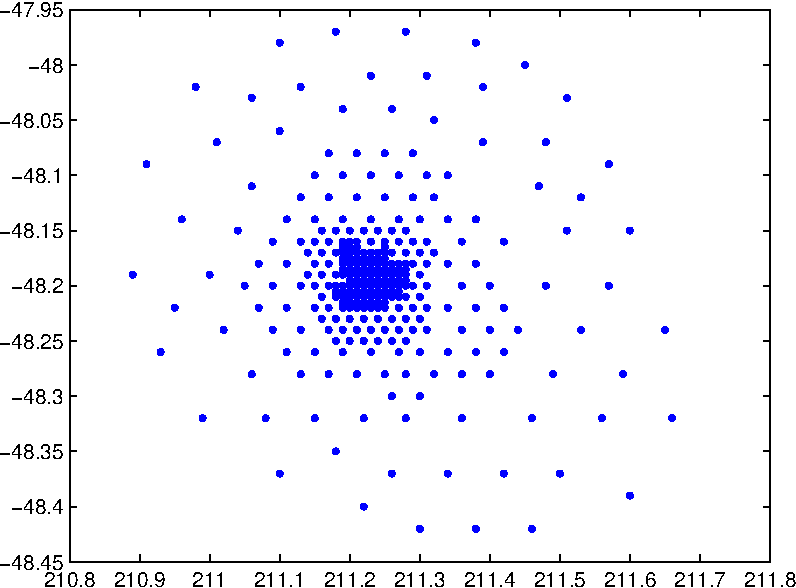
\includegraphics[width=0.6\textwidth]{figures/beispiel_scattered_data}
\end{center}
\end{frame}
%
% Slide
% 
\begin{frame}[fragile]\frametitle{Matlab: Beispiel}
\begin{matlabin}
xi = linspace(min(x),max(x),40);
yi = linspace(min(y),max(y),40);
[XI,YI] = meshgrid(xi,yi);
F = TriScatteredInterp(x,y,z,'linear');
ZI = F(XI,YI);
surf(XI,YI,ZI)
\end{matlabin}
\begin{center}
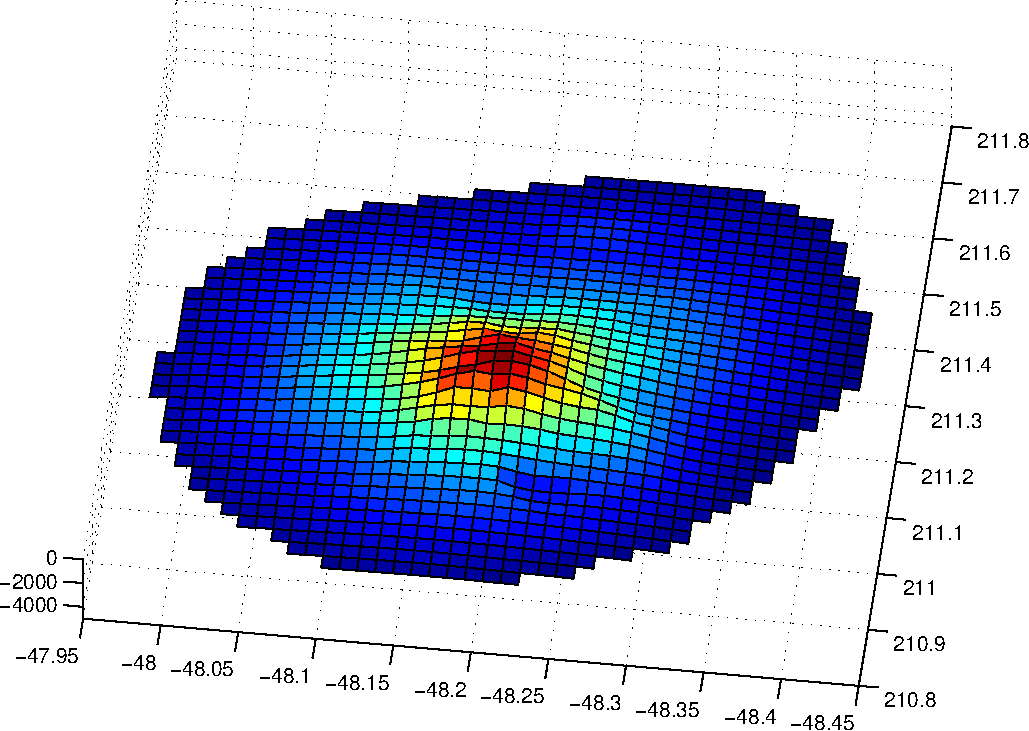
\includegraphics[width=0.6\textwidth]{figures/beispiel_scattered_data_plot}
\end{center}
\end{frame}

\begin{frame}[fragile]{Python: Beispiel}
\begin{pyin}
xi = linspace (min(x),max(x),40)
yi = linspace (min(y),max(y),40)
[XI ,YI] = meshgrid (xi ,yi)
ZI = sp.griddata ((x,y),z,(XI,YI),method='linear')
fig = figure() , ax = Axes3D(fig)
ax.plot_surface(XI ,YI ,ZI,rstride=1,cstride=1) 
\end{pyin}
\begin{center}
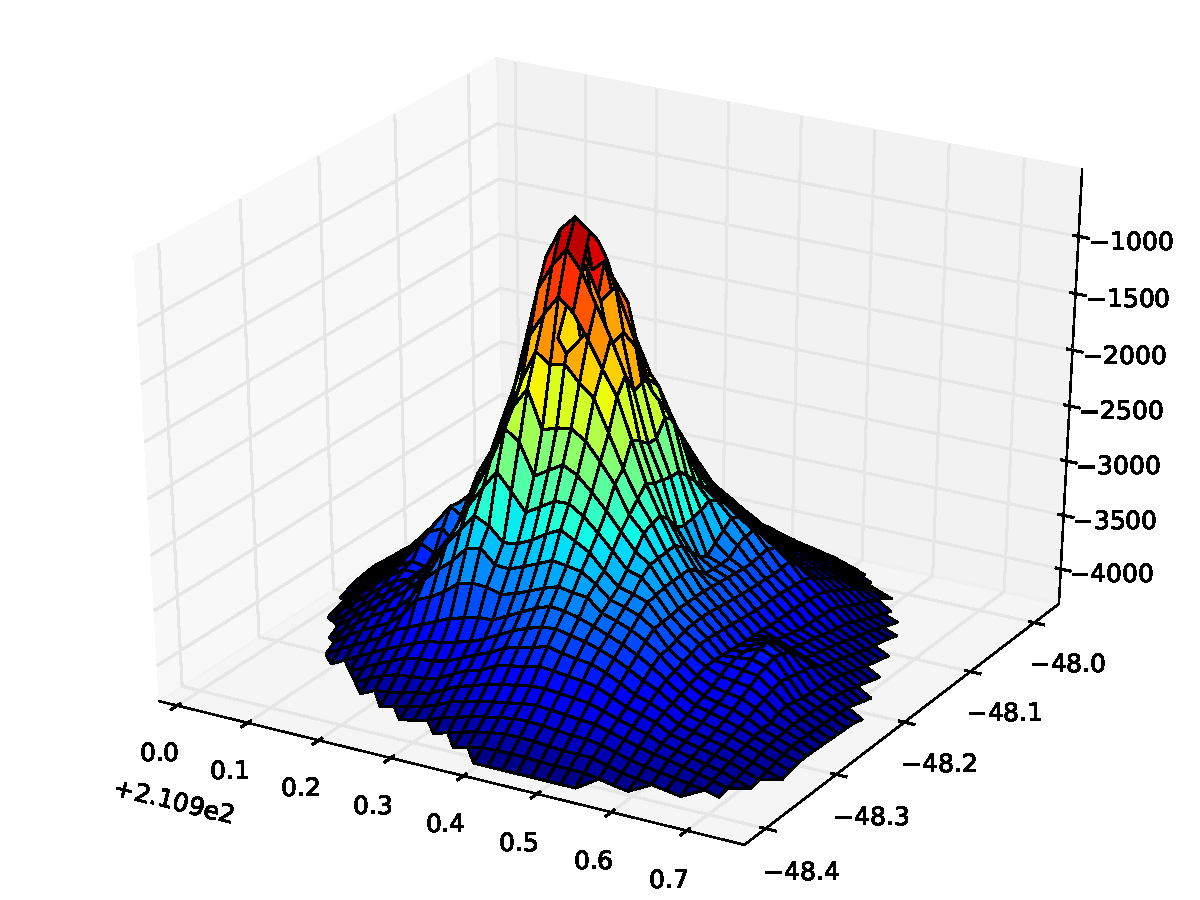
\includegraphics[width=0.5\textwidth]{figures/scattered_data_plot_py}
\end{center}
\end{frame}
%
% Slide
% 
\begin{frame}[fragile]\frametitle{Unstrukturierte Gitter Interpolieren}
\begin{matlabin}
F = TriScatteredInterp(<x>,<y>,<z>,<methode>);
ZI = F(<XI>,<YI>);
\end{matlabin}
\begin{pyin}
ZI = sp.interpolate.griddata ((<x>,<y>),<z>,(<XI>,<YI>),method='<methode>')  
\end{pyin}
\begin{itemize}
\item Vektoren $x,y,z$ enthalten Werte $(x(i),y(i),z(i))$.
\item Interpolationsstellen $(XI(i,j),YI(i,j))$ mit Matrizen \mcode{XI, YI}. 
\item (Matlab) Funktionsauswertung mit \mcode{F}: Ergebnis $ZI(i,j)$.
\item Art des Interpolierens:
\begin{itemize}
 \item \mcode{'nearest'}: st\"uckweise konstant
 \item \mcode{'linear'}: linear
% \item \mcode{'natural'}: natürliche Nachbarn (Voronoi-Diagramm)
\end{itemize}
\item Es wird nur innerhalb der konvexen H\"ulle der Punkte $(x(i),y(i))$
  interpoliert. Ansonsten Funktionswert \mcode{NaN}. 
\end{itemize}
\end{frame}

%
% Slide
% 
\begin{frame}[fragile]\frametitle{Matlab: Bemerkungen}
\begin{itemize}
\item Der Interpolation liegt eine \alert{Delaunay} Triangulation zugrunde. Die Werte
  $(x(i),y(i))$ sind Eckpunkte der entstehenden Dreiecksmenge.
\item Danach werden mit Hilfe der Dreiecke Funktionen  definiert, die
  entsprechende Werte besitzen. 
\item Mittels \mcode{TriScatteredInterp} ist die Technik auch auf h\"ohere Dimensionen
  anwendbar. Dreiecke werden durch entsprechende höher-dimensionale
  Simplizes ersetzt. \\
(In 3D: Tetraeder)
\end{itemize}
\end{frame}
%
% Slide
% 
\begin{frame}[fragile]\frametitle{Auf beliebigen Punkten Interpolieren}
\begin{matlabin}
ZI = interp2(<X>,<Y>,<Z>,<XI>,<YI>,<method>)
\end{matlabin}
\begin{pyin}
f=sp.interpolate.interp2d(<XI>,<YI>,<ZI>,kind='<method>')
ZI= f(XIp,YIp)
\end{pyin}
\begin{itemize}
\item Allgemein sind $X,Y,Z$ Matrizen. Dabei ist $Z(i,j)$ der Funktionswert an
  $(X(i,j),Y(i,j))$. $X$ und $Y$ sind in der Regel durch \mcode{meshgrid} erzeugt. 
\item Es wird an den Stellen $(XI(i,j),YI(i,j))$ interpoliert. Das Ergebnis
  ist $ZI(i,j)$. Die Einträge von $XI$ bzw. $YI$ k\"onnen beliebig sein. 
\item Art des Interpolierens (method):
\begin{itemize}
% \item \mcode{'nearest'}: st\"uckweise konstant
 \item \mcode{'linear'}: linear
 \item \mcode{'cubic'}: bikubische Splines
\end{itemize}
\end{itemize}
\end{frame}

%
% Slide
% 
\begin{frame}[fragile]\frametitle{Matlab: Interp2 - Beispiel}
\begin{matlabin}
xip = linspace(min(x),max(x),15); yip = linspace(min(y),max(y),15);
[XIp,YIp] = meshgrid(xip,yip);
ZIp = interp2(XI,YI,ZI,XIp,YIp,'linear');
surf(XIp,YIp,ZIp)
\end{matlabin}
\begin{center}
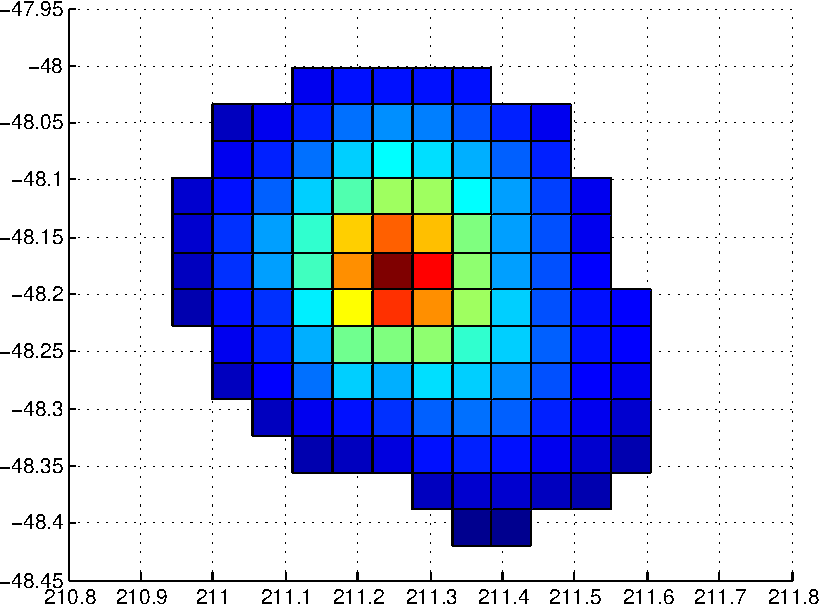
\includegraphics[width=0.6\textwidth]{figures/beispiel_interp2_plot}
\end{center}
\end{frame}

%
% Slide
% TODO: interp2 stuerzt mit den gegeben daten immer noch ab...
\begin{frame}[fragile]\frametitle{Python: Interp2 - Beispiel}
\begin{pyin}
xip = linspace (min(x),max(x),15), yip = linspace (min(y),max(y),15)
[XIp ,YIp] = meshgrid (xip ,yip)
f = inter.interp2d (xi,yi,ZI,kind='linear')  
ZIp = f(XIp,YIp)
\end{pyin}
%\begin{center}
%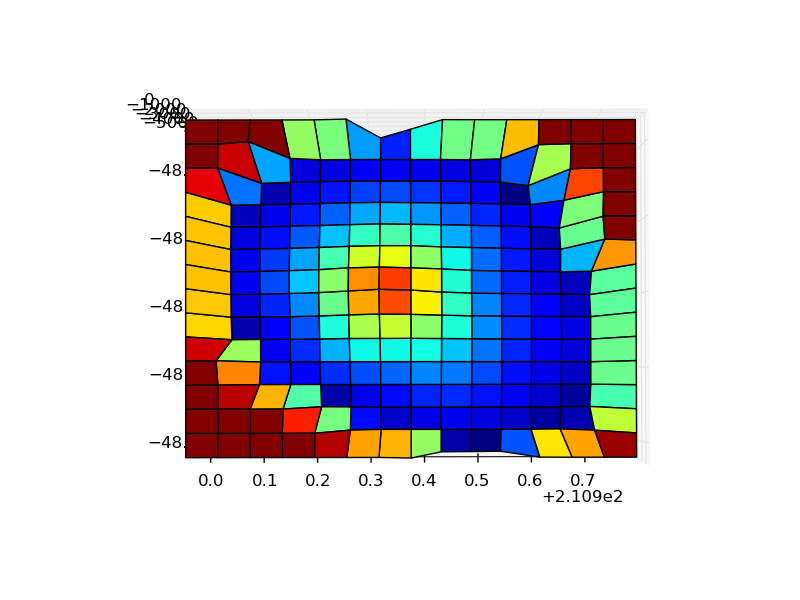
\includegraphics[width=0.6\textwidth]{figures/beispiel_interp2_pyplot}
%\end{center}
\end{frame}

\section{In- und Output}
%
% Slide
%
\begin{frame}[fragile]\frametitle{Input und Output}
\begin{itemize}
\item Benutzereingabe
\item einfache und formatierte Ausgabe
\item Schreiben in Dateien
\item Einlesen von Daten aus Dateien
\item Speichern und Laden von Variablen\\
\item Matlab: \alert{ \imatlab{help iofun}}: Übersicht über alle Ein- und  Ausgabe - Befehle
\end{itemize}
\end{frame}
%
% Slide
%
%\begin{frame}[fragile]\frametitle{Matlab: Benutzereingabe}
%\begin{itemize}
%\item Standardeingabe: 
%\begin{matlabin}
%input 
%\end{matlabin}
%\begin{pyin}
%raw_input()
%\end{pyin}
%%\item Eingabe eines Zeichens:
%\item Informationssteuerung durch die Maus:
%\begin{matlabin}
%ginput()
%\end{matlabin}
%
%\item Anhalten der Prozedur bis eine Tastatureingabe erfolgt: 
%\begin{matlabin}
%pause
%\end{matlabin}
%\begin{pyin}
%raw_input()
%\end{pyin}

%\end{itemize}
%\end{frame} 
%
% Slide
%
\begin{frame}[fragile]\frametitle{input}
\begin{matlabin}
ein = input('Text'[,'s'])
\end{matlabin}
\begin{pyin}
ein = raw_input('Text')  
\end{pyin}
Eingabe vom Benutzer abfragen und 'Text' anzeigen. Die Eingabe durch Return abschliessen. (Matlab: Option 's' erwartet ein String).

\begin{matlabin}
2*input('Bitte geben Sie den Startwert ein: ')
\end{matlabin}
\begin{pyin}
2*float(raw_input('Bitte geben Sie den Startwert ein: '))
\end{pyin}
\begin{matlab}
Bitte geben Sie den Startwert ein: 8
16.0
\end{matlab}
\begin{matlabin}
f = input('Eingabe einer Funktion: ', 's')
\end{matlabin}
\begin{pyin}
f = raw_input('Eingabe einer Funktion: ')
\end{pyin}
\begin{matlab}
Eingabe einer Funktion: sin(x)*cos(x)
f = sin(x)*cos(x)
\end{matlab}
\end{frame}
%
% Slide
%
\begin{frame}[fragile]\frametitle{ginput}
Das Kommando 
\begin{matlabin}
[x,y] = ginput(n)
\end{matlabin}
\begin{pyin}
coord = ginput(n)  
\end{pyin}
gibt die Koordinaten der $n$ Maus-Klicks als Vektoren $x$ und $y$ bzw. als Liste von xy-Tuplen zurück, 
an denen sich die Maus im aktuellen Grafik-Fenster befunden hat.  
\begin{itemize}
  \item \mcode{[x,y]=ginput}| \isage{ginput(0)} sammelt so lange Daten ein, bis die
  Return-Taste bzw. mittlere Maustaste gedrückt wird.
\item \mcode{[x,y,taste]=ginput(n)}(Matlab) gibt auch den Vektor \mcode{taste}
  zurück, der aus Werten $1$ (linke Maustaste), $2$ (mittlere
  Maustaste) oder $3$ (rechte Maustaste) besteht. 
\end{itemize} 
\end{frame}
%
% Slide
%
\begin{frame}[fragile]\frametitle{Bezier-Polynom}
\alert{ \[ z (t):=\sum_{i=0}^n {\bf b}_i B_i^n(t), \quad t \in [0,1] \]}
\begin{itemize}
\item $z(t): [0,1] \rightarrow \mathbb{R}^2$ ist das {\it Bezier-Polynom}.
\item ${\bf b}_i \in \mathbb{R}^2$ sind die vorgegebenen 
{\it Kontrollpunkte}.
\item $B_i^n(t)=\left( n \atop i \right) t^i (1-t)^{n-i}$ sind 
{\it Bernstein-Polynome}.
\end{itemize}
\end{frame}
%
% Slide
%
\begin{frame}[fragile]\frametitle{Matlab: Bezier-Polynom}
\begin{center}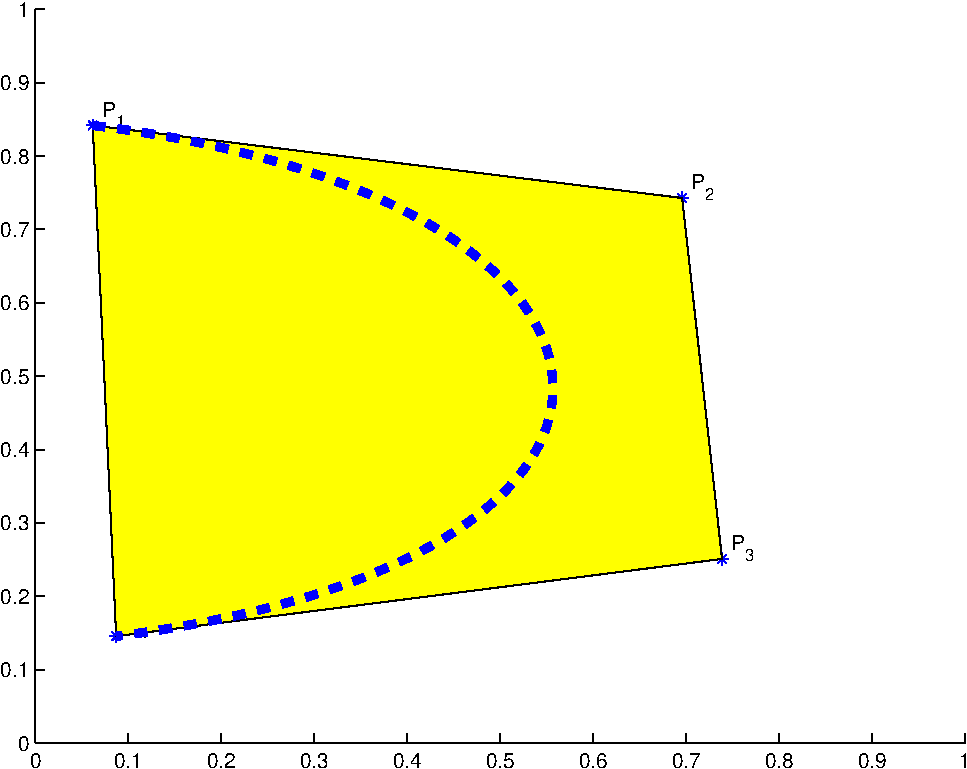
\includegraphics[width=0.8\textwidth]{figures/bezier}\end{center}
\end{frame}
%
% Slide
%
\begin{frame}[fragile]\frametitle{Matlab: Bezier-Polynom}
\matinput{bezier.m}
\end{frame}
%
% Slide
%
\begin{frame}[fragile]\frametitle{Python: Bezier-Polynom}
  \begin{pyin}
figure()
axis ([0,1,0,1])
x = zeros((4,))
y = zeros((4,))
for k  in range(0,4):
    p = ginput(2)
    x[k] = p[0][0]
    y[k] = p[0][1]
    plot(x[k],y[k],'*')
    text(x[k]+0.01 ,y[k]+0.01 , 'P_{}'.format(k) )
    draw()
# Zeichnen der Kontrollpolygons
fill(x,y,'y')
u = arange(0,1,0.01)
umat = array([(1 -u)**3, 3*u*(1 -u)**2, 3*u**2*(1-u), u**3 ])
plot(dot(x,umat) , dot(y,umat) ,'--',linewidth=4)
draw()    
  \end{pyin}
\end{frame}
%
% Slide
%
\begin{frame}[fragile]\frametitle{Matlab: Ausgabe}
\begin{itemize}
\item Text durch String-Aneinanderhängen
\begin{matlabin}
text=['Pi mit 5 signifikanten Stellen : ' num2str(pi,6)]
\end{matlabin} 
\begin{matlab} 
text =
Pi mit 5 signifikanten Stellen : 3.14159
\end{matlab} 
\item Ausgabe des Strings $X$ durch  \mcode{disp(X)}
\begin{matlabin}
disp(text)
\end{matlabin} 
\begin{matlab} 
Pi mit 5 signifikanten Stellen : 3.14159
\end{matlab} 
\item Ausgabe durch  \mcode{fprintf()}
\begin{matlabin}
fprintf('Pi mit %1.0f Nachkomma-Stellen : %6.4f \n',4,pi)
\end{matlabin} 
\begin{matlab} 
Pi mit 4 Nachkomma-Stellen : 3.1416 
\end{matlab}
\end{itemize}
\end{frame}
%
% Slide
%
\begin{frame}[fragile]\frametitle{Matlab: fprintf- Formartierte Ausgabe}
\begin{matlabin}
fprintf( <Format>, <Argument1>, <Argument2>,...)
\end{matlabin}
\textit{Format}: Output-Form der Argumente (Werte der Variablen): 
\begin{matlabin}
'.. %<(-|+)> <v1.n1><typ1> .. %<(-|+)> <v2.n2><typ2> ..'
\end{matlabin} 
\begin{description}
\item [<*>] Hier kann beliebiger Text eingegeben werden.
\item [<(-|+)>] '+': Vorzeichen-Anzeige erzwungen.\\
  '-': linksbündige Ausgabe.\\
 Weglassen von <(-|+)>: rechtsbündige Ausgabe ohne Anzeige des '+' Zeichens.
\item [v\textit{i}] Anzahl der insgesamt dargestellten Zeichen von Argument\textit{i}.
\item [n\textit{i}] Anzahl von Nachkommastellen. 
\item [typ\textit{i}] Datentyp und Darstellungsformat von Argument\textit{i}:
\begin{itemize}
 \item \alert{f} (Standarddarstellung von Gleitkommazahlen)
 \item \alert{e} (Expontialdarstellung von Gl.)
 \item \alert{g} (entweder Darst. $f$ oder $e$)
 \item \alert{s} (Strings),... 
\end{itemize}

\end{description}
\end{frame}
%
% Slide
%
\begin{frame}[fragile]\frametitle{Matlab: Bemerkungen zu fprintf}
\begin{itemize} 
\item Die formatierte Ausgabe ist an den Ansi-C Standard angelehnt.
\item Durch \mcode{'\\n'} wird ein Zeilenumbruch bewirkt. \mcode{'\\\%'} erzeugt
  \mcode{\%}.
 \item \mcode{sprintf} funktioniert wie \mcode{fprintf}. Allerdings wird
  die Ausgabe als String zurückgegeben. 
\item Ist ein Argument eine Matrix, so wird fprintf 'vektorisiert'.
\end{itemize}
\end{frame}

%
%
%
\begin{frame}[fragile]{Python: Formatierte Strings/Ausgabe}
  \begin{pyin}
'.. {<name|index>:<format>} .. {<name|index>:<format>} ... '.format(x,y,...) )
  \end{pyin}

  \isage{<format>}: [<flag>][<minwidth>][.<precision>]converter
  \begin{itemize}
    \item \emph{flag}: 0 für das Auffüllen mit Nullen
    \item \emph{minwidth}: Minimale Breite der Darstellung
    \item \emph{precision}: Genauigkeit (Nachkommastellen)
    \item \emph{converter}:
    \begin{itemize}
      \item \alert{d}   ganze Zahl mit Vorzeichen 
      \item \alert{e}  Gleitkommazahl mit Exponentialformat (kleingeschrieben) 
      \item \alert{f}   Gleitkommazahl im Dezimalformat 
      \item \alert{g}   Gleitkommazahl. Exponent $<$ -4: Exponentialform, Dezimalformat sonst
      \item \alert{s}   Strings  
    \end{itemize}
  \end{itemize}

\end{frame}

%
% Slide
\begin{frame}[fragile]\frametitle{Matlab: Schreiben in Dateien - Beispiel}
\matinput{waehrung.m}
\end{frame}
%
% Slide
\begin{frame}[fragile]\frametitle{Python: Schreiben in Dateien - Beispiel}
  \begin{pyin}
waehrung_name = raw_input('Umrechnung fuer welche Waehrung ?')
print('Ein Euro entspricht wievielen {} ? '.format(waehrung_name))
umrechnung = float(raw_input(''))
a = [1,2,3,5,10,20,50,100,200,1000]
fid = open('umrechnung.txt','w')
fid.write('Umrechnungstabelle: Euro-{}\n\n'.format(waehrung_name))
for i in a:
  fid.write('{:7.2f} Euro = {:7.2f} {}\n'.format(i,umrechnung*i,waehrung_name))
fid.write('\n\n Umrechnungskoeffizient: {:3.2f} \n'.format(umrechnung))
fid.close()    
  \end{pyin}
\end{frame}
%
% Slide
%
\begin{frame}[fragile]\frametitle{Datei öffnen}
\begin{matlabin}
fid = fopen(<dateiname>, <erlaubnis>)
\end{matlabin}
\begin{pyin}
fid = open(<dateiname>, <erlaubnis>)  
\end{pyin}

\mcode{fopen} öffnet die Datei \mcode{dateiname} im Modus
  \mcode{erlaubnis} und erzeugt einen
  Datei-Handle \mcode{fid}. Für \mcode{erlaubnis} gibt es u.a. die folgenden
  Möglichkeiten:
\begin{description}
\item ['r']  Lesen aus der Datei.
\item ['w']  Schreiben in die Datei (Erzeugen falls nötig)
\item ['a']  Hinzufügen (Erzeugen falls nötig)
\item ['r+'] Lesen und schreiben (aber nicht erzeugen) 
\end{description}
(Matlab) Durch ein  zusätzliches Output-Argument können Fehler aufgefangen
  werden. 
\begin{matlabin}
[fid, message]=fopen(<dateiname>, <erlaubnis>)
\end{matlabin}
Ist  die Datei nicht zu öffnen, so ist \mcode{fid=-1}. 
\end{frame}
%
% Slide
%
\begin{frame}[fragile]\frametitle{Weitere Kommandos}
\begin{itemize}
\item In Datei Schreiben
\begin{matlabin}
fprintf( <Datei-Handle>, <Format>, <Argument1>, <Argument2>,..)
\end{matlabin}
\begin{pyin}
fid.write('Text')
\end{pyin}
  \item \imatlab{fclose(fid)} | \isage{fid.close()} schliesst die Datei mit dem Handle \mcode{fid}
\end{itemize}
\end{frame}
%
% Slide
%
\begin{frame}[fragile]\frametitle{Matlab: Lesen aus einer Datei - Beispiel}
\matinput{waehrung_auslesen.m}
\end{frame}
%
% Slide
%
\begin{frame}[fragile]\frametitle{Matlab: fscanf formatiertes Lesen}
\begin{matlabin}
[daten,anz] = fscanf(<fid>,<format>,<Größe>)
\end{matlabin}
\begin{itemize}
\item \mcode{fscanf} liest Daten aus der Datei mit dem Handle
  \mcode{fid}. 
\item Die Daten werden in \mcode{daten} gespeichert. Der optionale Wert
  \mcode{anz} gibt die Anzahl erfolgreich gelesener Daten an.
\item \mcode{format} gibt das vorgegebene Suchmuster vor.
\item Die \mcode{Größe} bestimmt das was gelesen wird, und damit auch die Dimension der Output-Matrix. \mcode{inf} bezeichnet dabei das Dateiende.
\end{itemize}
\end{frame}
%
% Slide
%
\begin{frame}[fragile]\frametitle{Python: Lesen aus einer Datei - Beispiel}
  \begin{pyin}
#Datei einlesen
fid = open('umrechnung.txt','r')
fil = fid.read()
fid.close()
# Benutze regular Expressions um erste Zeile einzulesen
res = re.search('Umrechnungstabelle: Euro-(.*)',fil)
waehrung_name = res.group(1)
# regular expressions fuer alle Daten
daten = re.findall('([\d.]+) Euro =\s*([\d.]+)',fil)
# konvertieren der liste von tuples 
daten = array(daten,dtype=float)
# finden des Koeffizienten 
res = re.search('Umrechnungskoeffizient: ([\d.]+)',fil)
umrechnung = float(res.group(1))
#Ausgabe
print('Umrechnung: Euro - {}: Kurs: {} \n'.format(waehrung_name,umrechnung))
for x in daten:
    print(' {:7.2f} Euro  = {:7.2f}'.format(x[0],x[1]))    
  \end{pyin}
\end{frame}

%
% Slide
%
\begin{frame}[fragile]\frametitle{Python: Regular Expressions}
Regular expressions sind eine eigene Beschreibungssprache und sehr mächtig
zum Finden und evtl. Ersetzen in Strings (Module \isage{re}).

\begin{pyin}
reo = re.search(pattern, string)
\end{pyin}
Sucht im \isage{string} nach gegebenen Suchkriterien \isage{pattern}. Gibt RE-Objekt zurück falls die Suche erfolgreich ist, sonst \isage{None}
\begin{pyin}
liste = re.findall(pattern, string)
\end{pyin}
Sucht im \isage{string} nach gegebenen Suchkriterien \isage{pattern}. Gibt Liste aller gefundenen Stellen zurück.
\begin{itemize}
  \item \isage{reo.group(n)}: Gibt die $n$-te gefundene Gruppe als String wieder. $0$ ist der gesamte gefundene String.
\end{itemize}
\end{frame}
%
% Slide
%
\begin{frame}[fragile]\frametitle{Python: Regular Expressions - Kurzreferenz}

  \begin{itemize}
    \item \isage{.}: Findet jedes Zeichen.
    \item \isage{*}: Finde Zeichen, Zeichenklasse oder Gruppe keinmal oder beliebig oft.
    \item \isage{+}: Finde Zeichen, Zeichenklasse oder Gruppe einmal oder beliebig oft.
    \item \isage{(..)}: Gruppen. Alles was darin gefunden wird kann entsprechend der $n$-ten Gruppen abgefragt werden.
    \item \isage{[..]}: Klasse von Zeichen die gefunden werden können.
    \item \isage{\\d}: vordefinierte Klasse von Zeichen: alle Zahlen.
    \item \isage{\\s}: vordefinierte Klasse von Zeichen: alle Whitespaces (Leerzeichen, tabs, Returns)
  \end{itemize}
  Beispiel:
  \begin{pyin}
re.findall('([\d.]+) Euro =\s*([\d.]+)',fil)
  \end{pyin}
\end{frame}
%
% Slide
%
\begin{frame}[fragile]\frametitle{Python: loadtxt - Einlesen von Daten}
\begin{pyin}
array = np.loadtxt(fname,delimiter=None,comments='#')
\end{pyin}
\begin{itemize}
  \item \isage{fname}: Dateiname. 
  \item \isage{delimiter}: Trennzeichen. Z.B. ',' bei kommaseparierten Tabellen. Default-Einstellung sind Leerzeichen.
  \item \isage{comments}: Kommentarzeichen. In Python-Dateien z.B. '\#'.
  \item \isage{array}: Rückgabewert als (multidimensionaler) array.
\end{itemize}
Flexibleres Einlesen: \isage{np.genfromtxt()}
\end{frame}
%
% Slide
%
\begin{frame}[fragile]\frametitle{Weitere Befehle für das Einlesen}
\begin{itemize}
\item Zeile aus der Datei mit  Handle \mcode{fid} lesen und als String zurückgeben:
\begin{matlabin}
fgetl(fid) 
\end{matlabin}
  \begin{pyin}
fid.readline()
  \end{pyin}
\item Ganze Datei lesen und als String zurückgeben:
  \begin{pyin}
fid.read()
  \end{pyin}
\item Prüfen ob das Dateiende erreicht ist:
\begin{matlabin}
feof(fid)
\end{matlabin}
\mcode{feof(fid)} gibt eine $1$
  zurück, falls das Dateiende erreicht ist und $0$ sonst. (In Python nicht nötig)
\end{itemize}
\end{frame}
%
% Slide
%
\begin{frame}[fragile]\frametitle{Beispiel - Bubblesort}
\begin{itemize}
\item Bubblesort durchläuft die Datenmenge von Anfang bis zum Ende und
vergleicht paarweise die nebeneinanderstehenden Elemente. 
\item Sind zwei
benachbarte Elemente nicht in der richtigen Reihenfolge, so werden sie
miteinander vertauscht. 
\item Ist man am Ende angekommen, beginnt man wieder
von vorne. 
\item Die Datenmenge ist sortiert, falls bei einem Durchlauf
keine Vertauschungen mehr vorgenommen werden.
\end{itemize} 
\end{frame}
%
% Slide
%
\begin{frame}[fragile]\frametitle{Matlab: Bubblesort}
\begin{matlabin}
function sortieren(dateiname1, dateiname2)
% sortieren   Die Datei dateiname1 wird alphabetisch sortiert
%             und als dateiname2 abgespeichert.
%   INPUT:    STRING dateiname1
%             STRING dateiname2
 
% Datei laden
[fid,message] = fopen(dateiname1,'r');
if fid==-1 
    error('Datei nicht gefunden');
end;
% Datei lesen
anz = 0;
while feof(fid)==0
    anz = anz+1;     
    inhalt{anz}=fgetl(fid); 
end
fclose(fid);
\end{matlabin}
\end{frame}
%
% Slide
%
\begin{frame}[fragile]\frametitle{Matlab: Bubblesort (Forts.)}
\begin{matlabin}
% Sortieren
sortierungen = 1; 
while sortierungen>0
    sortierungen = 0;
    for k = 1:anz-1
        % vergleich_gr(a,b) ist 1 fuer a<b, 0 sonst
        if vergleich_gr(inhalt{k+1},inhalt{k})
            hilf = inhalt{k}; inhalt{k} = inhalt{k+1}; 
            inhalt{k+1} = hilf;
            sortierungen = sortierungen+1;
        end
    end
end
% Datei schreiben
fid = fopen(dateiname2,'w');
for k = 1:anz
   fprintf(fid,'%s \n',inhalt{k}); 
end;
fclose(fid);
\end{matlabin}
\end{frame}

\begin{frame}[fragile]{Python: Bubblesort}
  \begin{pyin}
def bubblesort(dateiname1, dateiname2):
   fid = open(dateiname1,'r')
   inhalt = []
   for line in fid:
       inhalt.append(line)
   fid.close()
   sortierungen = 1
   while sortierungen>0:
       sortierungen = 0
       for k in range(0,len(inhalt)-1):
           if vergleich_gr(inhalt[k+1],inhalt[k]):
               hilf = inhalt[k]
               inhalt[k] = inhalt[k+1]
               inhalt[k+1] = hilf
               sortierungen += 1
   fid = open(dateiname2,'w')
   for k in range(1,len(inhalt)):
       fid.write('{}'.format(inhalt[k]))
   fid.close()    
  \end{pyin}
\end{frame}

%
% Slide
%
\begin{frame}[fragile]\frametitle{Spezialisierte Einleseroutinen}
\begin{itemize}
%\item Es ist auch möglich temporäre Dateien zu erzeugen.
\item Binäre Dateien: (Matlab) \alert{\imatlab{fread}} und \alert{\imatlab{fwrite}}. (Python) open mit 'br' für <Erlaubnis>
%\item Excel-Tabellen lesen: \alert{\mcode{xlsread}} 
%\item Python: \isage{loadtext} \isage{savetext} kann viele Textformate Lesen/Schreiben.
\item Bilddateien: \alert{\imatlab{imread}/\imatlab{imwrite}} (SciPy)
\item Matlab: Audiodateien (.wav) bzw. Videodateien (.avi):
\alert{\imatlab{wavread}} bzw. \alert{\imatlab{aviread}}. 
\item Python: \isage{io.video.Video}
 \item Matlab-Dateien: \imatlab{save} \imatlab{load}| \isage{scipy.io.savemat} \isage{scipy.io.loadmat}
\end{itemize}
\end{frame}
%
% Slide
%%
%\begin{frame}[fragile]\frametitle{Matlab:  Bin\"are Daten}
%\begin{matlabin}
%%-------------------- beispiel_bin_data.m
%A = hilb(10);
%
%% Schreibe binaere Datei
%fwriteid = fopen('hilb10.bin','w');
%count = fwrite(fwriteid,A,'double');
%fclose = (fwriteid);
%
%% Lesen binaere Datei
%freadid = fopen('hilb10.bin','r');
%B = fread(freadid, count, 'double');
%C = reshape(B,10,10);
%
%disp(norm(A - C))
%\end{matlabin}
%\end{frame}
%
% Slide
%
%\begin{frame}[fragile]\frametitle{Laden und Speichern von  Variablen}
%\begin{itemize}
%\item \alert{ \mcode{save filename}} speichert den gesamten
%  Workspace in der Datei \mcode{filename.mat}. Einladen des Workspace
%  ist möglich mittels  \alert{ \mcode{load filename}}. 
%\item Mittels \alert{ \mcode{save filename A x}} werden nur die
%  Variablen $A$ und $x$ in der Datei \mcode{filename.mat}
%  gespeichert. Durch  \alert{ \mcode{load filename}} werden nun die
%  Variablen $A$ und $x$ dem Workspace hinzugefügt. 
%\item Bei \mcode{load} werden bestehende Variablen mit dem gleichen
%  Namen überschrieben.
%\end{itemize}
%\end{frame}

\section{Etwas Debugging}
%
% Slide
%
\begin{frame}[fragile]\frametitle{Fehler-Arten}
\begin{itemize}
\item \alert{ Syntax Fehler}: z.B. Schreibfehler oder
  Weglassen von Klammern. Die meisten dieser Fehler werden im Editor angezeigt. 
  und werden ansonsten als entsprechende Fehlermeldung ausgegeben. 
\item \alert{ Run-time Fehler}: Diese Fehler sind
  normalerweise algorithmischer Natur. Oft passen z.B. bei
  Matrixoperationen die Matrizen nicht zusammen.
\end{itemize}

\scriptsize{ Die erste Fehlermeldung zeigt bei geschachtelten Funktionsaufrufen
an, in welcher Funktion der Fehler liegt.}
\end{frame}
%
% Slide
%
\begin{frame}[fragile]\frametitle{Matlab: Fehler abfangen}
\begin{itemize}
\item \alert{Fehlermeldungen}
\begin{matlabin}
error(<text>) 
\end{matlabin}
Bricht das Programm ab. Insbesondere die Eingabeparameter sollten auf Fehler geprüft werden.
\item \alert{Warnungen}
\begin{matlabin}
warning(<text>)
\end{matlabin}
Programm wird fortgesetzt.
\end{itemize}
\end{frame}
%
% Slide
%
\begin{frame}[fragile]\frametitle{Matlab: Beispiel}
\begin{matlabin}
function interpolation(f1,N)
\end{matlabin}
\alert{ \centering{$\cdots$}}\\
\begin{matlabin}
%----------------- Fehlerbehandlung
if (round(abs(N)) ~= N) | (N==0)
    error(strcat('Bitte fuer die Anzahl der Stuetzstellen',...
    'eine natuerliche Zahl verwenden'));
end
if ~ischar(f1)
    error('Bitte fuer die Funktion einen String verwenden');
end
\end{matlabin}
\end{frame}

\begin{frame}[fragile]\frametitle{Matlab: Integrierter Debugger}
\begin{itemize}
 \item \alert{Breakpoints}: Halten das Programm an der Gegebenen Stelle an. Aktivierung: Klick in der linken Spalte rechtes neben der Zeilennummer. 
 \item \alert{Debug-Modus}: Menu: Debug->Stop if Errors/Warnings auf \textit{always stop if error} setzen.
 \item \alert{Step} (F10) Ein Schritt weiter im gegebenen Kontext.
 \item \alert{Step in} (F11) Ein Schritt weiter im gegebenen Kontext. Wechselt zu aufgerufenen Funktionen. 
\item \alert{continue} (F5) Führt das Programm normal fort.
\end{itemize}
\end{frame}


\begin{frame}[fragile]\frametitle{Python: Integrierter Debugger}
\begin{itemize}
  \item \alert{Breakpoints}: Halten das Programm an der gegebenen Stelle an. Setzen der Stelle: (F12) in der jeweiligen Zeile.
  \item \alert{Debug-Lauf}: (STRG+F5) Startet das Programm im Debugger und hält z.B. an Breakpoints an.
\end{itemize}
Debugger-Befehle:
\begin{itemize}
  \item \isage{up} Eine Funktionsebene hochgehen.
  \item \isage{down} Eine Funktionsebene runtergehen.
  \item \isage{next} Ein Schritt weiter im gegebenen Kontext.
 \item \isage{step} Ein Schritt weiter im gegebenen Kontext. Wechselt zu aufgerufenen Funktionen. 
\item \isage{cont} Führt das Programm normal fort (bis zum nächsten Breakpoint). Auch ganz am Anfang notwendig damit Programm startet.
\item \isage{!command} Python-Befehl ausführen die sich mit Debugger-Befehlen überschneiden. Ansonsten kann man direkt Python-Befehle ausführen und so auch die lokalen Variablen analysieren.
\end{itemize}
\end{frame}






\end{document}

